    % ---------------------------------------------------------------------
    % ---------------------------------------------------------------------
    % ---------------------------------------------------------------------

    \chapter{Entrenament de models acústics}
    \label{cap03__}

    % ---------------------------------------------------------------------
    % ---------------------------------------------------------------------
    % ---------------------------------------------------------------------

    % Procediment (recepta explicada)
    %
En el present capítol es descriu el procediment i les tècniques emprades per l'entrenament de models acústics híbrids de tipus BLSTM-HMM.
Inicialment, la Secció~\ref{cap03_intro} resumeix el procés seguit per generar un model acústic.
A continuació, la Secció~\ref{cap03_prepro} explica els passos necessaris per preparar les dades que s'empraran durant els entrenaments dels diferents models.
En tercer lloc, la Secció~\ref{cap03_gmmhmm} descriu el procediment que cal seguir per entrenar un model GMM-HMM.
La Secció~\ref{cap03_dnnhmm} explica com entrenar un model FF-DNN-HMM.
Finalment, la Secció~\ref{cap03_blstmhmm} detalla com entrenar un model BLSTM-HMM.
 
\section{Introducció}
\label{cap03_intro}

El procediment d'entrenament de models híbrids està dividit principalment en tres fases.
La Figura~\ref{fig:resum_am} mostra, de manera esquemàtica, aquestes fases.
Primerament, s'entrena un model acústic de tipus GMM-HMM, consistent en un model ocult de Markov inicial, en el que les probabilitats d'emissió dels estats es modelen amb una mixtura de Gaussianes. Aquest model s'usa a continuació per a inicialitzar i entrenar un model híbrid FF-DNN-HMM. De la mateixa manera, aquest segon model es fa servir per a inicialitzar el tercer i últim model BLSTM-HMM.

L'aproximació d'entrenar models auxiliars ve motivada pel fet que la BLSTM no pot entrenar-se directament. 
Per poder modelar $P(q_t|\textbf{x}_t)$ amb una BLSTM, necessitem obtindre les etiquetes $q_t$ associades a cada vector acústic d'entrada $\textbf{x}_t$, és a dir, necessitem els alineaments més probables $(q_t, \textbf{x}_t), \; \in {1,T}$.
Açò s'obté inicialment amb el model auxiliar GMM-HMM, ja que permet modelar directament $P(\textbf{x}_t|q _t)$ sense cap prerequisit previ amb un model generatiu com són les mixtures de Gaussianes.
Amb les dades alineades d'aquest model, és a dir, amb els diferents vectors de característiques emparellats als senones que representen, podem entrenar una xarxa neuronal, en aquest cas una FF-DNN. 
La raó per entrenar una FF-DNN i no passar directament a una BLSTM és perquè les FF-DNN donen alineaments més precisos, de millor qualitat, per entrenar el model final BLSTM-HMM, gràcies a la seua capacitat discriminativa i la seua robustesa front a soroll i possibles \textit{outlayers}, és a dir, frames incorrectament alineats pel model GMM-HMM.
%En el cas que tinguérem ja un model entrenat i amb les dades alineades, podríem botar-nos aquesta part de la tasca. De fet, aquest mateix sistema podrà ser reentrenat amb dades noves mitjançant l'alineament de les seues dades en un futur si fora necessari.

    \begin{figure}[h]
        \centering
        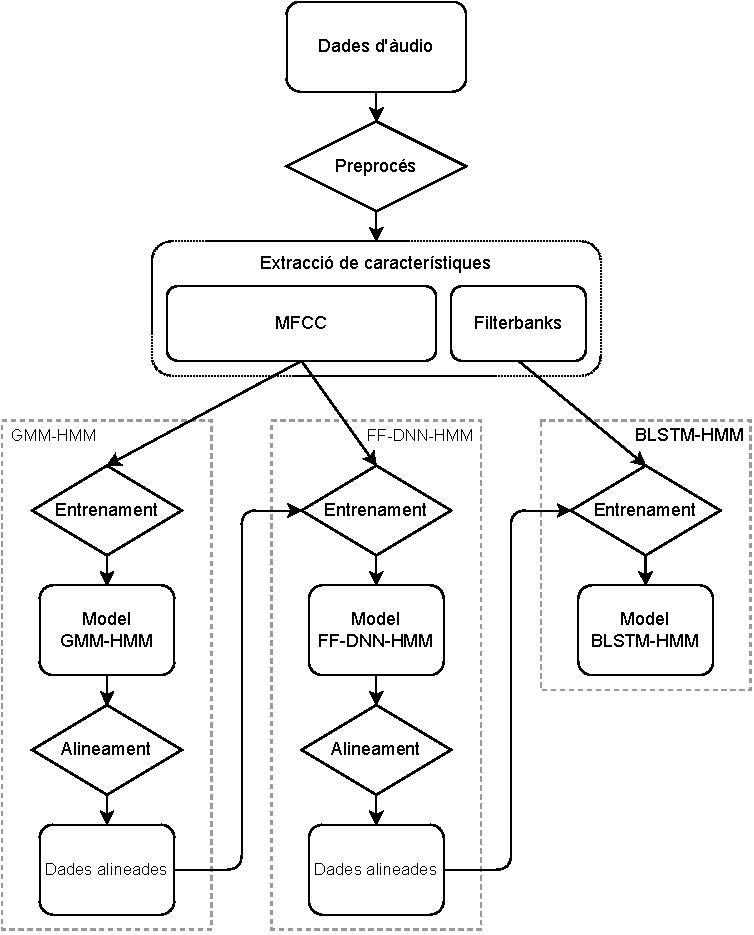
\includegraphics{figuras/resum_am.pdf}
        \caption{Diagrama que mostra els diferents passos seguits per a la creació del model acústic.}
        \label{fig:resum_am}
    \end{figure}

\section{Preprocés i extracció de característiques}
\label{cap03_prepro}

En primer lloc, quant al preprocés, s'apliquen una sèrie de transformacions sobre el text de les transcripcions de la parla per eliminar informació que no afecta a la pronunciació, ja que encara que siguen correctes, aquestes presenten una varietat d'informació que és irrellevant per a obtenir la correcta pronunciació de les mostres: majúscules, signes de puntuació o dígits.
A continuació, es genera una transformació de paraules a seqüència de fonemes, usant un diccionari de pronunciació o model lèxic, generat de forma manual amb coneixement expert, o de forma automàtica mitjançant models estadístics~\cite{BISANI2008434}.

En segon lloc, pel que respecta al pas d'extracció de característiques, s'aplica el procés descrit a la Secció~\ref{cap02_preprocessat_acustic} per a extreure vectors de característiques de tipus MFCC per a l'entrenament dels models GMM-HMM i FF-DNN-HMM, i de tipus Filterbank per a l'entrenament del model final BLSTM-HMM. 


\section{Entrenament de GMM-HMM}
\label{cap03_gmmhmm}

Les raons per entrenar un model GMM-HMM són, per una banda, obtenir una topologia de senones, és a dir, definir el conjunt de classes del model acústic; i per altra banda, aconseguir un alineament de les dades d'entrenament per poder entrenar un model acústic neuronal de majors prestacions en passos posteriors.
    
Aquest procés requereix un conjunt de mostres d'entrenament dels vectors de característiques MFCC, junt a les seues transcripcions fonètiques.
Per entrenar els HMMs, usarem l'algorisme d'expectativa-maximització Baum-Welch, algorisme iteratiu que optimitza els paràmetres d'un model amb variables ocultes. És a dir, es tracta de descobrir els camins $q$ que millor expliquen les seqüències d'observacions $x$ d'entrenament.
Les taules de transicions seran reutilitzades pels diferents models especificats ací.

Primer s'entrenen HMMs de monofonemes amb Gaussianes diagonals, inicialitzades amb l'estimació d'una única Gaussiana global amb la mitjana i la variància dels frames d'entrenament.
En aquest cas, cada HMM modela un únic monofonema, però per necessitat d'identificar el context immediat s'introdueixen els trifonemes. Un trifonema, com el seu nom indica, és un conjunt de tres fonemes: el central, que dona la informació principal i és vertader fonema a identificar, i els laterals, que afegeixen el context necessari per a una millor classificació del fonema central. D'aquesta manera, un trifonema sol definir-se com $S_1-S_2+S_3$, on $S_2$ és el fonema central, a ser identificat, i ambdós $S_1$ i $S_3$ el seu context esquerre i dret, respectivament.

A continuació, s'entrenen HMMs de trifonemes amb Gaussianes diagonals, sent inicialitzats amb els paràmetres del monofonema central del model anterior.
No obstant, els models HMMs de trifonemes presenten un problema important. Posem d'exemple el Francés, una llengua amb 35 fonemes. Aquests generen potencialment 42875 trifonemes diferents, cadascun amb tres estats. Això implica un total de 128625 estats, tots i cadascun d'ells equipats amb una Gaussiana o mixtura de Gaussianes. A més, durant l'entrenament hi haurà trifonemes que apareixeran poques vegades o que directament no existeixen en el corpus de train.
Aquests problemes es solucionen mitjançant l'algorisme CART, que ens permet detectar i agrupar estats de HMMs de diferents trifonemes amb poca o nu\lgem a observació estadística que son similars des d'un punt de vista estadístic. Així, estats agrupats s'uneixen per conformar un únic estat nugat (\textit{tied-state}) compartit per múltiples models de HMMs de trifonemes lligats.
%Algunes de les preguntes que es realitzen durant la creació d'aquest arbre són \guillemotleft està a la dreta/esquerra hi ha una vocal?\guillemotright o \guillemotleft està a principi de paraula?\guillemotright.
%L'arbre CART es crea de forma automàtica mitjançant un script amb un set de regles que fa totes les preguntes bàsiques possibles a ambdós costats (dreta i esquerra) i una sèrie de preguntes extra per a casos particulars de la llengua. 
Per a una explicació més detallada del CART, així com de possibles tècniques per optimitzar-lo, es recomana a la lectora dirigir-se a \cite[cap. 18.1]{pml1Book}.

Una vegada generat el conjunt d'estats nugat, s'inicialitza el model de trifonemes nugats amb Gaussianes diagonals, on cada Gaussiana obté el valor inicial de la Gaussiana que representa la seua fulla de l'arbre CART, emprant les mateixes taules de transicions. Aquest model s'entrena amb diverses iteracions de l'algorisme de EM.

Finalment, s'entrena el model GMM-HMM de trifonemes lligats, amb Mixtures de Gaussianes diagonals. Aquest és un procés iteratiu i molt costós, doncs cada model utilitza l'anterior per a entrenar-se. S'entrenen diferents models, cadascun amb una mixtura de $2^i : 0 \le i \le N$ components per cada estat nugat del model, on $N$ es un paràmetre a fixar.

Com s'ha introduït a l'inici del capítol, és necessari obtenir alineaments dels frames d'entrenament a nivell d'estat de model HMM per poder entrenar el model FF-DNN-HMM. 
Per aconseguir-ho, s'usa el model GMM-HMM definitiu de trifonemes lligats amb mixtures de Gaussianes, el qual calcula la seqüència d'estats $\hat{q}$ del model de Markov que millor explica cadascuna de les mostres $\textbf{x}$ d'entrenament. Convé destacar que la seqüència d'estats $\hat{q}$ revel·la la seqüència de trifonemes que, d'acord amb el model acústic, millor descriu l'observació acústica $\textbf{x}$.

    
\section{Entrenament de FF-DNN-HMMs}
\label{cap03_dnnhmm}

En aquest pas, es reutilitza la topologia (conjunt d'estats i probabilitats de transició) del model GMM-HMM. Sols s'entrena la FF-DNN encarregada de modelar $P(q_t|\textbf{x}_t)$, tal i com s'ha detallat en la Secció~\ref{cap02_asr_am}

La FF-DNN té en l'eixida una capa softmax amb tantes neurones com senones té el model acústic. Aquesta s'entrena diverses èpoques amb els alineaments de la GMM-HMM del pas anterior fins arribar a convergència, contro\lgem ant l'error de classificació (FER) calculat sobre el conjunt de \textit{development}. Finalment, amb la FF-DNN entrenada, aquesta s'utilitza per calular uns nous alineaments frame-senone més acurats, aprofitant la potència discriminativa de la FF-DNN front a la GMM, per usar-los en l'últim pas per entrenar la BLSTM.


\section{Entrenament de BLSTM-HMM}
\label{cap03_blstmhmm}
De manera similar al model FF-DNN-HMM, s'entrena una xarxa BLSTM per modelar $P(q_t|\textbf{x}_t)$ amb els alineaments calculats per la FF-DNN, que s'espera que siga encara millor que l'anterior gràcies a les particularitats de la xarxa recurrent: disposa de ce\lgem es LSTM que permeten mantenir informació i el reconeixement de mostres és teòricament superior, ja que aquest mecanisme de memòria permet mantindre un context.
De nou, s'entrena fins a la convergència controlant el FER en \textit{development}.
